% ==========================================================================================================================
\section{Arquitectura básica de SNMP}
% ==========================================================================================================================

\noindent
El modelo de administración de red que se utiliza para SNMP incluye los siguientes elementos:
\begin{itemize}
	\item Estación de gestión,
	\item Agente de Gestión,
	\item Base de información de gestión y
	\item Protocolo de Gestión de redes.
\end{itemize}

\noindent
En las secciones se enlistan las tareas para realizar la instalación y configuración de dichos elementos

% ==========================================================================================================================
\subsection{Instalación de la estación de gestión “Observium” en una máquina virtual}
% ==========================================================================================================================

\noindent
Para realizar la instalación de Observium sobre la máquina virtual debe tenerse previamente instalado un software de virtualización, para el caso utilizamos Virtual Box, así como la imagen ISO del sistema Observium a instalar. 

\noindent
\newline
\textbf{Paso 1:} Configuramos la red de la máquina virtual de Ubuntu, para eso debemos elegir el adaptador tipo puente, y dentro de las opciones avanzadas elegir el modo promiscuo. Como se ve a continuación: 

\pagebreak
\begin{figure}[htbp!]
	\centering
		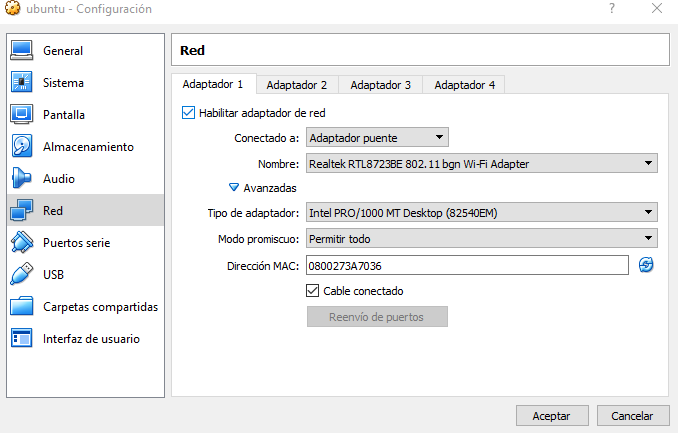
\includegraphics[width=0.8\textwidth]{images/desarrollo/instalarObservium_paso1.png}
	\caption{Instalación de observium: Paso 1.}
\end{figure}

\noindent
\textbf{Paso 2:} De las opciones de Virtual Box seleccionamos ''Almacenamiento'', luego ''Controlador IDE y seleccionamos la imagen ISO del sestema Observium. Como se muestra debajo: 

\begin{figure}[htbp!]
	\centering
		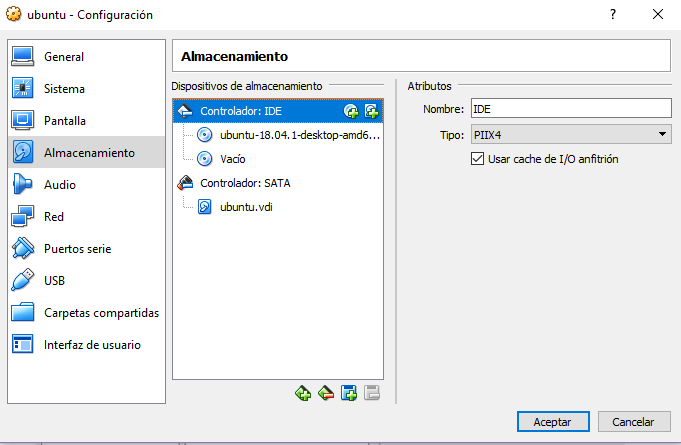
\includegraphics[width=0.8\textwidth]{images/desarrollo/instalarObservium_paso2.png}
	\caption{Instalación de observium: Paso 2.}
\end{figure} 

\pagebreak
\noindent
\textbf{Paso 3:} Creamos una nueva máquina virtual, e introducimos nombre, tipo y versión del sistema operativo a instalar. 

\begin{figure}[htbp!]
	\centering
		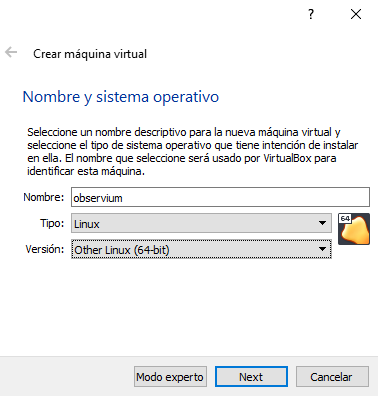
\includegraphics[width=0.5\textwidth]{images/desarrollo/instalarObservium_paso3.png}
	\caption{Instalación de observium: Paso 3.}
\end{figure} 

\noindent
\textbf{Paso 4:} Seleccionamos las características que tendrá nuestra máquina virtual para el sistema Observium. Tales como la memoria RAM o la capacidad de Disco duro. Como se muestra en las imágenes debajo. 

\begin{figure}[htbp!]
	\centering
		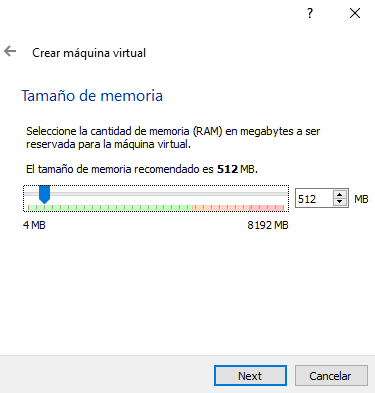
\includegraphics[width=0.5\textwidth]{images/desarrollo/instalarObservium_paso4a.png}
	\caption{Instalación de observium: Paso 4a.}
\end{figure} 

\pagebreak
\begin{figure}[htbp!]
	\centering
		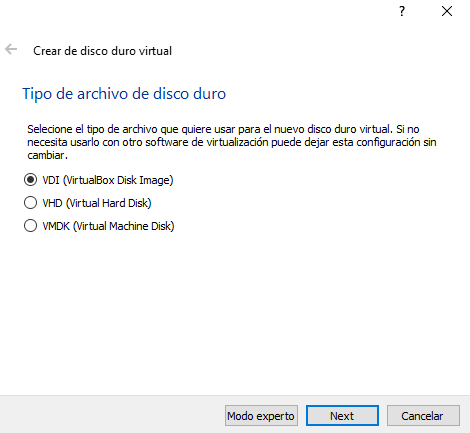
\includegraphics[width=0.5\textwidth]{images/desarrollo/instalarObservium_paso4b.png}
	\caption{Instalación de observium: Paso 4b.}
\end{figure} 

\noindent
\textbf{Paso 5:} Configuramos el adaptador de red, con las configuraciones que se observan en la imagen siguiente. 

\begin{figure}[htbp!]
	\centering
		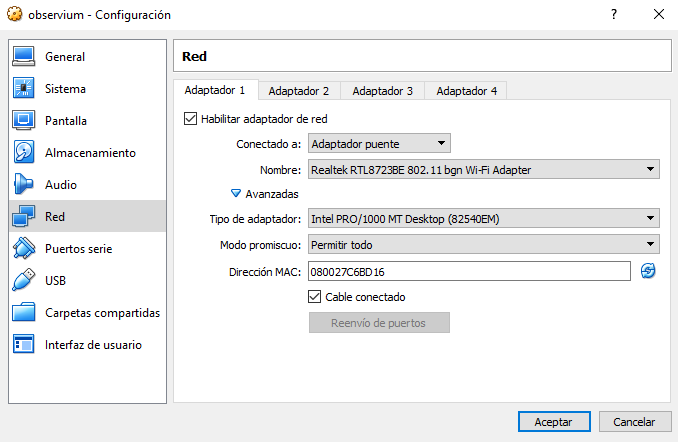
\includegraphics[width=0.8\textwidth]{images/desarrollo/instalarObservium_paso5.png}
	\caption{Instalación de observium: Paso 5.}
\end{figure} 

\noindent
\textbf{Paso 6:} Se selecciona la imagen ISO con la cual va a correr el sistema.

\pagebreak
\begin{figure}[htbp!]
	\centering
		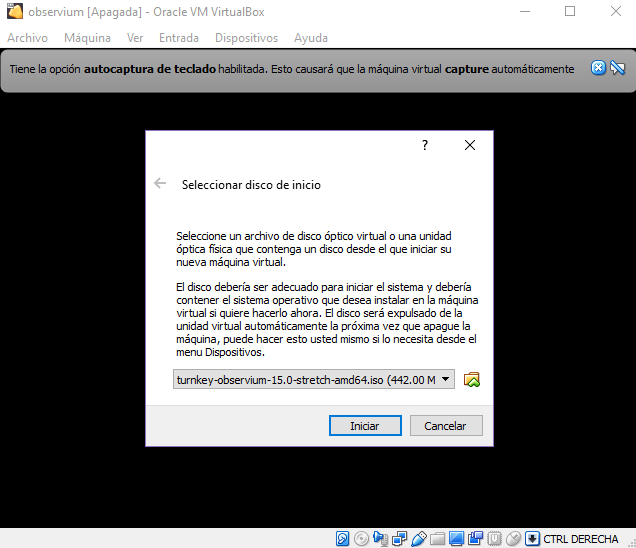
\includegraphics[width=0.6\textwidth]{images/desarrollo/instalarObservium_paso6.png}
	\caption{Instalación de observium: Paso 6.}
\end{figure}

\noindent
\textbf{Paso 7:} Seleccionamos la opción de ''instalar'' mostrada en la siguiente pantalla. 

\begin{figure}[htbp!]
	\centering
		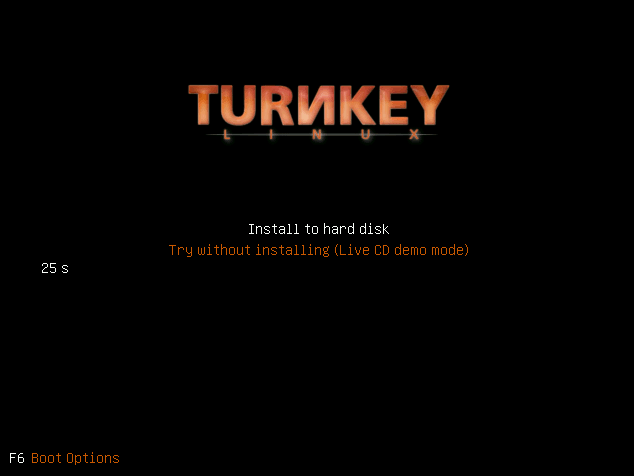
\includegraphics[width=0.8\textwidth]{images/desarrollo/instalarObservium_paso7.png}
	\caption{Instalación de observium: Paso 7.}
\end{figure}

\noindent
\textbf{Paso 8:} De las pantallas a continuación siga el flujo, seleccionando las opciones marcadas. 

\pagebreak
\begin{figure}[htbp!]
	\centering
		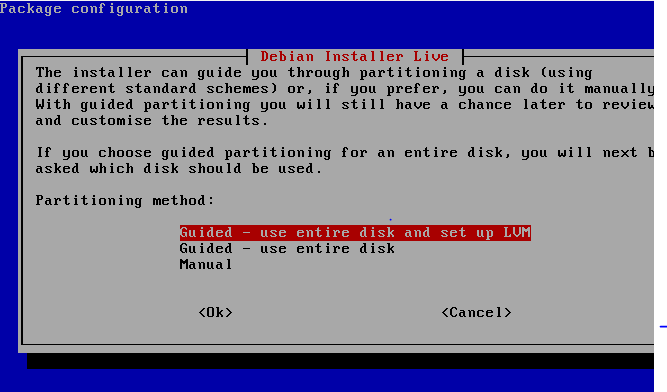
\includegraphics[width=0.8\textwidth]{images/desarrollo/instalarObservium_paso8.png}
	\caption{Instalación de observium: Paso 8.}
\end{figure}

\begin{figure}[htbp!]
	\centering
		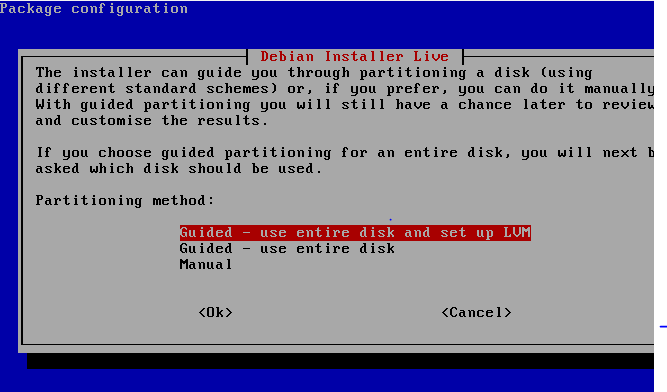
\includegraphics[width=0.8\textwidth]{images/desarrollo/instalarObservium_paso8.png}
	\caption{Instalación de observium: Paso 8.}
\end{figure}

\begin{figure}[htbp!]
	\centering
		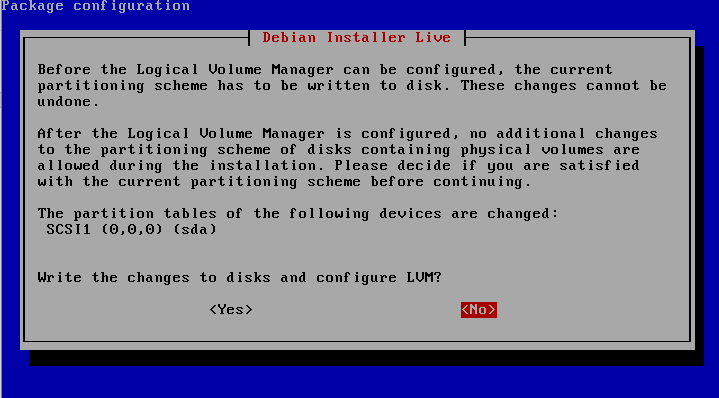
\includegraphics[width=0.8\textwidth]{images/desarrollo/instalarObservium_paso8b.png}
	\caption{Instalación de observium: Paso 8b.}
\end{figure}

\begin{figure}[htbp!]
	\centering
		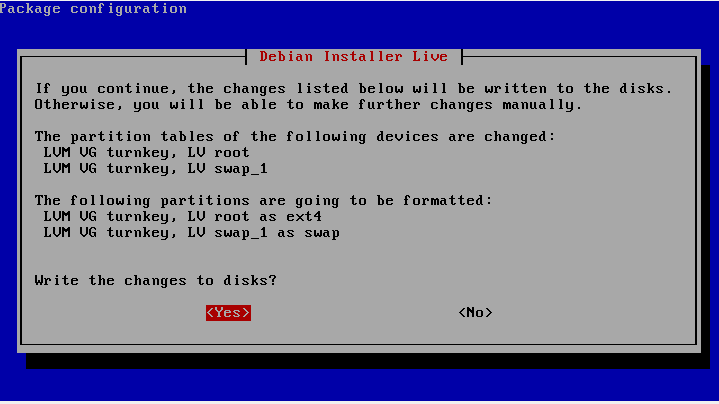
\includegraphics[width=0.8\textwidth]{images/desarrollo/instalarObservium_paso8c.png}
	\caption{Instalación de observium: Paso 8c.}
\end{figure}

\begin{figure}[htbp!]
	\centering
		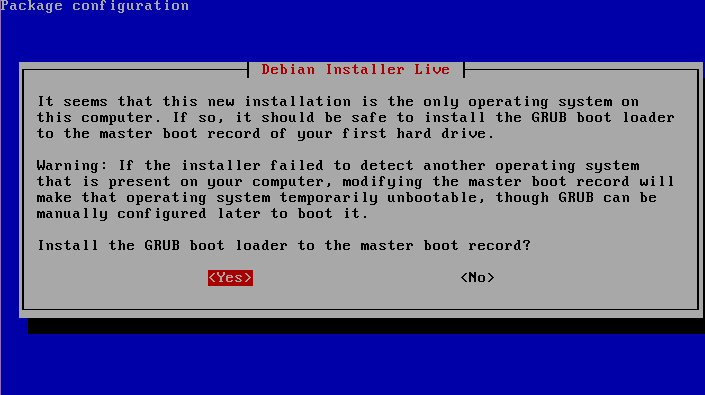
\includegraphics[width=0.8\textwidth]{images/desarrollo/instalarObservium_paso8d.png}
	\caption{Instalación de observium: Paso 8d.}
\end{figure}

\begin{figure}[htbp!]
	\centering
		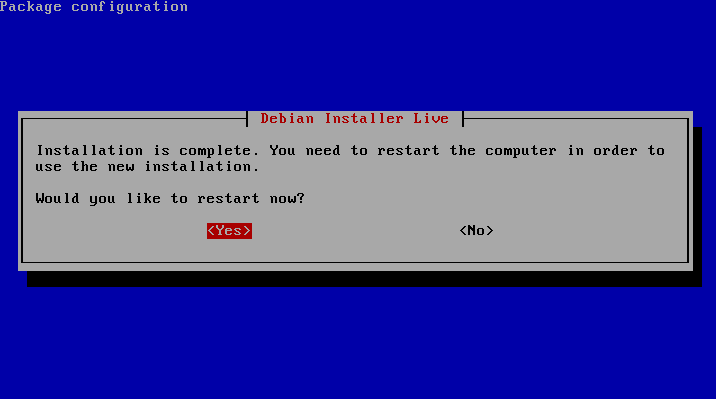
\includegraphics[width=0.8\textwidth]{images/desarrollo/instalarObservium_paso8e.png}
	\caption{Instalación de observium: Paso 8e.}
\end{figure}

\pagebreak
\noindent
\textbf{Paso 9:} Se establecen las contraseñas para la cuenta y la base de datos, así como un correo electrónico, como se observa en las imágenes debajo. 

\begin{figure}[htbp!]
	\centering
		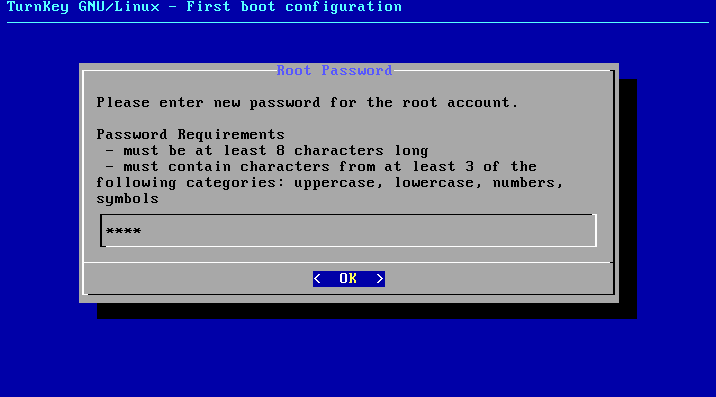
\includegraphics[width=0.8\textwidth]{images/desarrollo/instalarObservium_paso9a.png}
	\caption{Instalación de observium: Paso 9a.}
\end{figure}

\begin{figure}[htbp!]
	\centering
		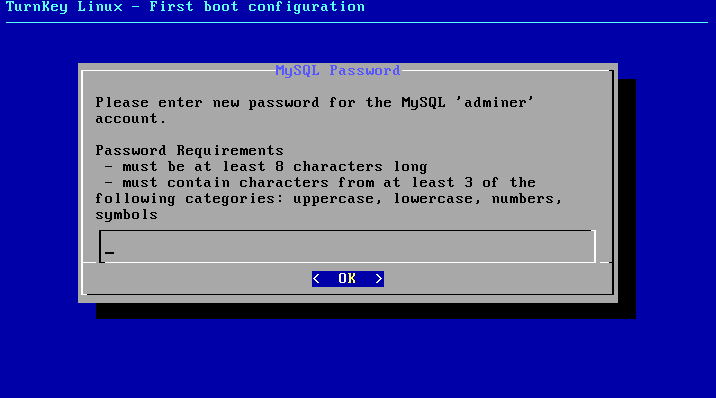
\includegraphics[width=0.8\textwidth]{images/desarrollo/instalarObservium_paso9b.png}
	\caption{Instalación de observium: Paso 9b.}
\end{figure}

\begin{figure}[htbp!]
	\centering
		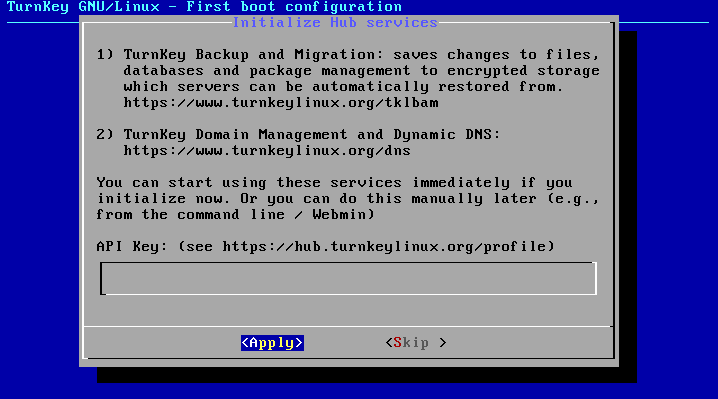
\includegraphics[width=0.8\textwidth]{images/desarrollo/instalarObservium_paso9c.png}
	\caption{Instalación de observium: Paso 9c.}
\end{figure}

\begin{figure}[htbp!]
	\centering
		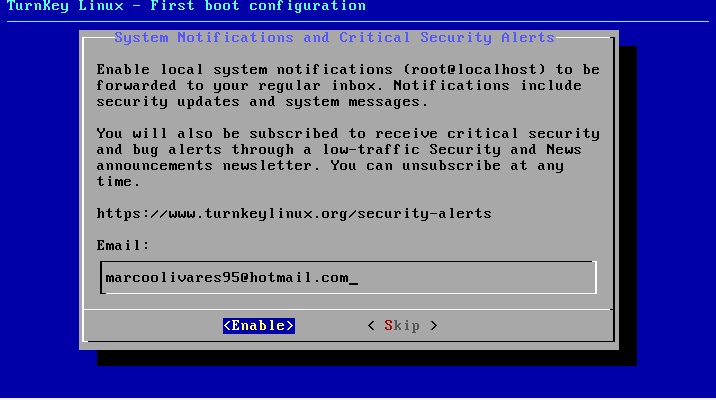
\includegraphics[width=0.8\textwidth]{images/desarrollo/instalarObservium_paso9d.png}
	\caption{Instalación de observium: Paso 9d.}
\end{figure}

\pagebreak
\noindent
\textbf{Paso 10:} Se selecciona la opción ''instalar'' y posteriormente ''reboot''. Como se muestra a continuación.

\begin{figure}[htbp!]
	\centering
		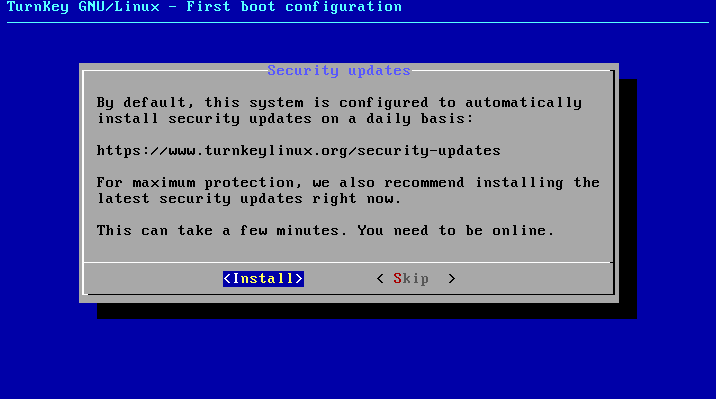
\includegraphics[width=0.8\textwidth]{images/desarrollo/instalarObservium_paso10a.png}
	\caption{Instalación de observium: Paso 10a.}
\end{figure}

\begin{figure}[htbp!]
	\centering
		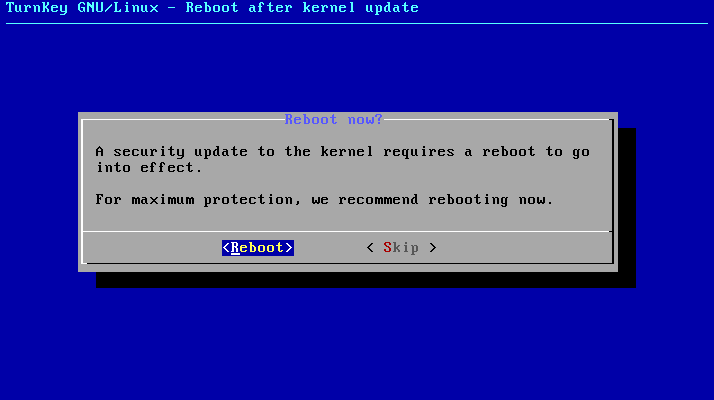
\includegraphics[width=0.8\textwidth]{images/desarrollo/instalarObservium_paso10b.png}
	\caption{Instalación de observium: Paso 10b.}
\end{figure}
